% ---
% Casa de Edmundo Guimarães ainda de pé
% ---

\afterpage{
\begin{figure}[!h]
\centering
\caption{Antiga casa de Edmundo Guimarães na ladeira dos Galés (2017)}
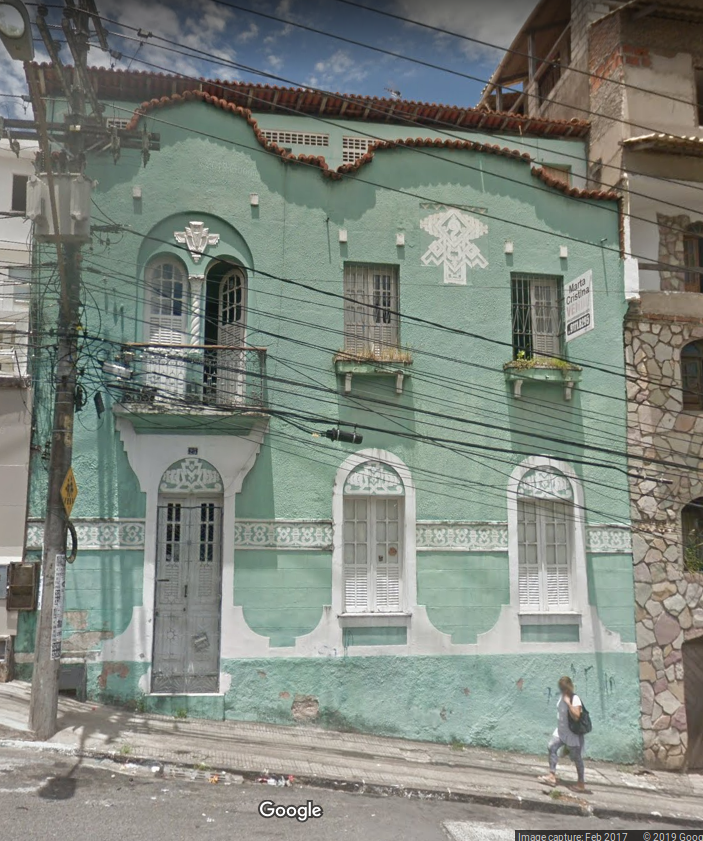
\includegraphics[width=1\textwidth]{8-anexos/plantas/01-1distrito/12-gales/ladeiradosgales-edmundoguimaraes-casa2017.jpg}{\footnotesize \par \textbf{Fonte:} Google Maps. }
\label{fig:edmundoguimaraes2017}
\end{figure}
}

% ---
% Casa de Maria Rosa Vianna Ferraz ainda de pé
% ---

\afterpage{
\begin{figure}[!h]
\centering
\caption{Antiga casa de Maria Rosa Vianna Ferraz, na rua do Castro Neves (2017). }
\includegraphics[height=0.9\textheight]{8-anexos/plantas/01-1distrito/16-castroneves/mariarosaviannaferraz-83e81-2017.jpg}{\footnotesize \par \textbf{Fonte:} Google Maps. }
\label{fig:mariarosaviannaferraz2017}
\end{figure}
}

% ---
% Casa de Domingos Gonçalves Cavalheiros na rua do Castro Neves, ainda de pé
% ---

\afterpage{
\begin{a3paisagem}
\begin{figure}[!htp]
	\caption{Casa de Domingos Gonçalves Cavalheiro, na rua do Castro Neves, em dois tempos}
	\centering
		\begin{subfigure}[t]{0.4\textwidth}
			\includegraphics[width=1\textwidth]{8-anexos/plantas/01-1distrito/16-castroneves/castroneves240-domingosgoncalvescavalheiro-1927.jpg}
			\caption{\footnotesize Projeto de Pedro Jayme David (1927). \textbf{Fonte:} \textbf{BR BAAHMS}, Fundo ``Intendência'', Série ``Processos de Licenciamento de Reforma e Ampliação de Edificações'', Subsérie ``Requerimentos e Plantas -- Brotas'', caixa 16. }
			\label{fig:domingosgoncalvescavalheiro-1927}
		\end{subfigure}
		\
		\begin{subfigure}[t]{0.4\textwidth}
			\includegraphics[width=1\textwidth]{8-anexos/plantas/01-1distrito/16-castroneves/castroneves240-domingosgoncalvescavalheiro-2017.jpg} 
			\caption{\footnotesize  O mesmo imóvel em 2017. \textbf{Fonte:} Google Maps. }
			\label{fig:domingosgoncalvescavalheiro-2017}
		\end{subfigure}
	\label{fig:domingosgoncalvescavalheiro}
\end{figure}
\end{a3paisagem}
}

% ---
% Casa de José Veríssimo Alves ainda de pé
% ---

\afterpage{
\begin{figure}[!h]
\centering
\caption{Antiga casa de José Veríssimo Alves, na rua do Sangradouro (2017). }
\includegraphics[width=1\textwidth]{8-anexos/plantas/01-1distrito/15-sangradouro/sangradouro-joseverissimoalves-2019n169.jpg}{\footnotesize \par   \textbf{Fonte:} Google Maps. }
\label{fig:joseverissimo2017}
\end{figure}
}

% ---
% Casa de Manoel Amoedo y Amoedo, na Uruguaiana, ainda de pé
% ---

\afterpage{
\begin{figure}[!h]
\centering
\caption{Antiga casa de Manoel Amoedo y Amoedo na esquina da rua Frederico Costa com a rua Boa Vista de Brotas (2016)}
\includegraphics[width=\textwidth]{8-anexos/plantas/02-boavista/01-uruguayana/2016-manoelamoedoyamoedo-casa.jpg}{\footnotesize \par \textbf{Fonte:} Google Maps. \par Curiosamente, no mesmo lugar demarcado no projeto para um ``armazém'' funciona ainda hoje uma padaria, e no lugar destinado aos ``bilhares'' funcionam hoje duas pequenas lojas. Não foi possível descobrir, mesmo em visita ao local, o que foi feito do andar nobre.}
\label{fig:2016-manoelamoedoyamoedo-casa}
\end{figure}
}

% ---
% Armazém Europa, na Waldemar Falcão, ainda de pé
% ---

\afterpage{
\begin{a3paisagem}
\begin{figure}[!h]
\centering
\caption{Antigo Armazém Europa, na esquina da rua Waldemar Falcão com a avenida D. João VI (2016)}
\includegraphics[height=0.9\textheight]{8-anexos/plantas/03-estbrotas/22-cruzdasalmas/2016-armazemeuropa.jpg}{\footnotesize \par \textbf{Fonte:} Google Maps. \par Embora a planta deste imóvel não tenha sido encontrada, a planta para a construção de uma bomba de gasolina pela Standard Oil (\textbf{BR BAAHMS}, Fundo ``Intendência'', Série ``Processos de Licenciamento de Reforma e Ampliação de Edificações'', Subsérie ``Requerimentos e Plantas -- Brotas'', caixa 22) indica a existência deste estabelecimento. Embora aparente drástica descaracterização, o estilo das portas é compatível com o de outras casas comerciais construídas no período estudado. }
\label{fig:2016-armazemeuropa}
\end{figure}
\end{a3paisagem}
}